\begin{homeworkProblem}
% \textbf{Virtual Initialization}. One problem with arrays is that they must typically be initialized prior to use. On most computing environments, when we allocate an array of O(n) words of memory they start out filled with “garbage” values (whatever data last occupied that block of memory), and we must spend O(n) time setting the words in the block to some initial value. In this problem, we wish to design a data structure that behaves like an array (i.e., allowing us to retrieve the ith value and modify the ith value both in O(1) time), but which allows for initialization to a specified value v in O(1) time as well. That is, if we ask for the value of an element we have not modified since the last initialization, the result should be v. The data structure should occupy O(n) space in memory (note that this could be twice or three times as large as the actual space we need to store the elements of the array), and the data structure should function properly regardless of whatever garbage is initially present in this memory. As a hint, try to combine the best features of an array and a linked list.
    % Give an appropriate positive constant \(c\) such that \(f(n) \leq c \cdot
    % g(n)\) for all \(n > 1\).

    % \begin{enumerate}
    %     \item \(f(n) = n^2 + n + 1\), \(g(n) = 2n^3\)
    %     \item \(f(n) = n\sqrt{n} + n^2\), \(g(n) = n^2\)
    %     \item \(f(n) = n^2 - n + 1\), \(g(n) = n^2 / 2\)
    % \end{enumerate}
\textbf{Requirements}
    \begin{enumerate}
        \item Retrieve the $ith$ value and modify the $ith$ value both in O(1) time
        \item Initialization to a specified value v in O(1) time
        \item Space: O(n), can twice or three times as large as the actual space we need.
        \item The data structure should function properly regardless of whatever garbage is initially present in the memory.
    \end{enumerate}
\textbf{Analyze}

We need to build a supplemental data structure to help us to do virtual initialization. Firstly, we add an n-element array B to record whether the value of an element we have modified since the last initialization.
\textbf{Initialization:} Create the n-element  array $B$. Time complexity: O(n)

\textbf{Read from A[i]}: Time complexity: O(1)

    \begin{enumerate}
        \item If $B[i]$ is off
            \begin{enumerate}
                \item Set $B[i]$ on
                \item Initialize $A[i] = v$
            \end{enumerate}
        \item Read $A[i]$
    \end{enumerate}

\textbf{Write to A[i]:}Time complexity: O(1)W
    \begin{enumerate}
        \item Set $B[i]$ on
        \item Write $A[i]$
    \end{enumerate}

However, if we only use an extra n-element array B to record whether we have modified the value from the last initialization. We can retrieve the ith value and modify the ith value both in O(1) time. But, we can't implement the initialization to a specified value v in O(1) time because we need to build the array $B$ firstly which is spent O(n) time. So, we try to add a queue $q$ which can record that which index has been modified after the last initialization.

\textbf{Initialization:} We empty the queue $q$ (change the q address), it means there is no element has been changed from the last initialization. Time complexity: O(1)

\textbf{Read from A[i]}: Time complexity: O(1)
    \begin{enumerate}
        \item If $B[i]$ != the front address of q
            \begin{enumerate}
                \item Push index i to queue q 
                \item Set $B[i]$ = the front address of q
                \item Initialize $A[i] = v$
            \end{enumerate}
        \item Read $A[i]$
    \end{enumerate}

\textbf{Write to A[i]:} Time complexity: O(1)
    \begin{enumerate}
        \item If $B[i]$ != the front address of q
            \begin{enumerate}
                \item Push index i to queue q 
                \item Set $B[i]$ = the front address of q 
                \item Initialize $A[i] = v$
            \end{enumerate}
        \item Write $A[i]$
    \end{enumerate}

Then the queue q has record all the index of the modified elements in the array A. We can check the queue to get all of them if we want to know which elements have been changed from last initialization.




\end{homeworkProblem}

\pagebreak

\begin{homeworkProblem}
% \textbf{Enumerating Subsets by Incrementing a Binary Counter}. This is a somewhat classical amortized analysis problem. Suppose we store the digits of an n-bit binary number B in an array A of length n. We wish to increment B from 0 to $2^n - 1$ while continually modifying the contents of A to reflect the digits in B. For example, if n = 3, then we will start with $A = (0, 0, 0)$, then we toggle the last entry to obtain A = (0, 0, 1). The next increment operation changes A to A = (0, 1, 0), and so on, until we finally reach A = (1, 1, 1). Please describe how to implement the operation increment that takes an array A and modifies it by incrementing its associated binary number. Although your operation will require $\theta(n)$ time in the worst case, please show that its amortized running time is only $O(1)$ (assuming the entries in A all start out at zero). Please show how to use the accounting method as well as a potential function to perform this amortized analysis.

\textbf{Requirements}
    \begin{enumerate}
        \item Describe how to implement the operation increment
        \item Show the amortized running time in only $O(1)$ (Assum the entries in A all start out at zero)
        \item Show how to use the accounting method as well as a potential function to perform this amortized analysis.
    \end{enumerate}

\textbf{Analyze}

We store the digits of an n-bit binary number B to count the incrementing and store this number to an array A of length n. And this increment counter is initially 0. The only operation is $increment(A)$. The worst case running time occurs when all k bits are flipped to 1, so $increment(A)$ has running time $O(k)$. Suppose we do $m$ increments, we choose $m = 9$ as an example.

\begin{center}
\begin{tabular}{|c|c|c|c|c|c|c|c|c|c|c|} %l(left)居左显示 r(right)居右显示 c居中显示
\hline 
Incrementing(op\#) & 0 & 1 & 2 & 3 & 4 & 5 & 6 & 7 & 8 & ...\\
\hline 
A & (0) & (1) &(1,0) & (1,1) & (1,0,0) & (1,0,1) & (1,1,0) & (1,1,1) &(1,0,0,0) & ...\\
Flipped Number & 0 & 1 & 2 & 1 & 3 & 1 & 2 & 1 & 4 & ... \\
Cumulative & 0 & 1 & 3 & 4 & 7 & 8 & 10 & 11 & 15 & ...\\
Total(Amortized) & 2 & 2 & 2 & 2 & 2 & 2 & 2 & 2 & 2 & ... \\
New Cumulative  & 2 & 4 & 6 & 8 & 10 & 12 & 14 & 16 & 18 & ...\\

\hline 
\end{tabular}
\end{center}

In this case, the total costs are about 2m which average is 2 units per increment. Then the amortized cost per operation is O(1).

\textbf{Aggregate Method for k-increments:} K-increment for each bits:
    \begin{enumerate}
        \item bit 0 flips with every increment
        \item bit 1 flips with every $2^{nd}$ increments
        \item bit 2 flips with every $4^{th}$ increments
        \item So, the bit k flips with every $(2^k)^{th}$ increments
    \end{enumerate}
So the total number of bit flips in k increment operations is: 

$Total\  op = k + k/2 + k/4 ...+ k/2^k = k*(1 + 1/2 + 1/4 + ... + 1/2^k) = 2k$ 

As a result, the total cost of the sequence is O(n), then the amortized cost per operation is $O(n) / n = O(1)$$. 

\textbf{Accounting Method for k-bit:} The actual cost for an increment operation is the number of bits
flipped. We can assign an amortized cost of 2 for each increment operation. The main idea is to use 1 to flip the bit from 0 to 1 and store 1 credit to flip it back to 0 later. All changes from 1 to 0 are paid for with previously stored credit. The amortized time per operation is O(1). 

\textbf{Potential Method:} Potential Function [1] $C_i = number$ of 1s in counter after $i^{th}$ increment. And we suppose $i^{th}$ operation resets $t_i$ bits to 0.

Actual cost: $c_i = t_i + 1$

And: $C_i \leq C_{i-1} - t_i + 1$. 
\begin{enumerate}
    \item If $C_i = 0, then \  C_{i-1} = t_i = k$.  
    \item If $C_i > 0, then \ C_i = C_{i-1} - t_i + 1$.  
\end{enumerate}

Difference in Potentials:

$C_i - C_{i-1} \leq (C_{i-1} - t_i + 1) - C_{i-1} = -t_i + 1$

As a result, the amortized cost for each operation: $c_i + C_i - C_{i-1} \leq (t_i + 1) - t_i + 1 = 2$

Then the amortized cost is O(1)

\end{homeworkProblem}



\begin{homeworkProblem}
% \textbf{Enumerating Permutations.} Consider a length-n array A = (1, 2, 3, . . . , n). We would like to step through all $n!$ permutations of A, updating the array as we go to represent each subsequent permutation. Permutations should be generated in lexicographic order; for example, with n = 3 we start with A = (1, 2, 3), then move to A = (1, 3, 2), A = (2, 1, 3), A = (2, 3, 1), A = (3, 1, 2), and finally A = (3, 2, 1). Please describe how to implement an operation next-perm with $O(1)$ amortized running time that modifies A to produce the next permutation in lexicographic order.Use a potential function in your analysis.
    % Write part of \alg{Quick-Sort($list, start, end$)}

\textbf{Requirements}
    \begin{enumerate}
        \item Describe how to implement an operation $next-perm$ with O(1) amortized running time that modifies A to produce the next permutation in lexicographic order.
        \item Use a potential function in the analysis.
    \end{enumerate}

\textbf{Analyze}

In order to find the next-perm base on the current number, we deal with this number from right to left. We define the index i and j $(i < j)$. For each index i, we want to find the first i which have $A[i+1] > A[i]$. After that, we try to search in the $A[i+1, ...., len]$ to find the $A[j] > A[i]$. Then swap A[i] with A[j] and reverse the A[i+1, ... n]. This operation will take n - i + 1 times. 

\begin{lstlisting}[language=C++]
vector<int>& nextPermutation(vector<int>& A) {
  unsigned len = A.size() - 1;
  // Find an element from the right to left.
  for (int i = len - 1; i >= 0; --i) {
    if (A[i + 1] > A[i]) {
      for (int j = len; j > i; --j) {
        if (A[j] > A[i]) {
          swap(A[j], A[i]);
          reverse(A.begin() + i + 1, A.end());
          return A;
        }
      }
    }
  }
  // If there are increate order from left to right.
  reverse(A.begin(), A.end());
  return A;
}
\end{lstlisting}

As the above code, there are a few steps to find the next permutation in lexicographic order. 
\begin{enumerate}
    \item Find the largest index $i$ such that $A[i] < A[i+1]$. If no such index exists, this is the last permutation, then reverse the array A to the first permutation.
    \item Find the largest index $j$ in the $[i+1, len]$ such that $A[j] > A[i]$
    \item Swap $A[i] \  with \  A[j]$
    \item Reverse the sequence from $A[i+1]$ up to and including the final element $A[len]$
\end{enumerate}

\textbf{Potential Method:} Define the potential function $\phi = number \ of \ descending  \ elements$ for index $i+1$ to n. And we suppose $i^{th}$ operation have $k$ elements in the descending elements were affected.

\begin{enumerate}
    \item Actual work: $W_i = k$.
    \item $\phi_i = k$
    \item $\phi_i \leq \phi_{i-1} - (k-2) + 1$
    \item Difference in Potentials: $\phi_i - \phi_{i-1} = - (k-2) + 1$
    \item The amortized cost for each operation: $W_k + \phi_i - \phi_{i-1} \leq k - (k-2) + 1 = 3$.
\end{enumerate}
Then the amortized cost is O(1)

\end{homeworkProblem}

\pagebreak

\begin{homeworkProblem}
% \textbf{In-Place Matrix Transposition.} Suppose we store an $m*n$ matrix in row-major form as an array of length $N = m*n$ in which we list the elements of the matrix one row at a time from left to right. By taking the transpose of such a matrix, we convert it into column-major form - an array of length N listing the columns of the matrix one at a time, each one from top to bottom. Suppose the matrix is sufficiently large that we would like to permute its memory representation from row-major to column-major order in place (using only $O(1)$ extra storage beyond the memory that holds the matrix). Please describe and analyze a $O(N log N )$ algorithm for solving this problem. As a hint, try to design an approach modeled on the “domination radius” algorithm from lecture, noting that for each element in the matrix, you can easily determine the location to which it needs to move, as well as the location of the element that will replace it.



\textbf{Requirements}
    \begin{enumerate}
        \item Suppose the matrix is sufficiently large that we would like to permute its memory representation from row-major to column-major order in place(Space Complexity: $O(1)$).
        \item Use a $O(NlogN)$ algorithm for solving this problem.
        \item Try to design an approach modeled on the "domination radius" algorithm.
    \end{enumerate}

\textbf{Analyze}

We store an m*n matrix in row-major form as an array of length N=m*n. And transport this matrix. We use an matrix A as an example.  \\
\begin{figure}[h]
\centering
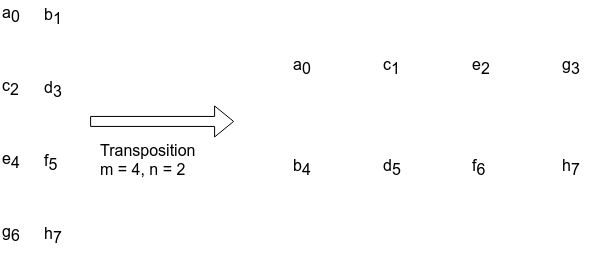
\includegraphics[scale=0.7]{images/1.png}
\end{figure}

In the above graph, small number at the right of the letter represent the index for the letter in the arrow. We can find the movement for this transposition like followed.
\begin{lstlisting}
Index movement:
0 -> 0
1 -> 4 -> 2 -> 1
2 -> 1 -> 4 -> 2(Repetition)
3 -> 5 -> 6 -> 3
4 -> 2 -> 1 -> 4(Repetition)
5 -> 6 -> 3 -> 5(Repetition)
6 -> 3 -> 5 -> 6(Repetition)
7 -> 7
\end{lstlisting}
These index movement are 4 cycle. $0->0$,  $1 -> 4 -> 2 -> 1$, $3 -> 5 -> 6 -> 4$ and $7 -> 7$. After that, we need to think about how to find whether the cycle is repetitive cycle and how to calculate the precursor and successor element for the current element. \\

\textbf{Solution}

\textbf{How to know the cycle is not repetitive?}

It is easy to find whether this cycle is a repetitive cycle because we traverse this array for index 0 to N. So the first index for a new cycle which is not a repetitive one should has the lowest first index in this cycle. As a result, the cycle is a repetitive cycle if there is a successor index is bigger than the first index in the cycle. 
\begin{lstlisting}[language=C++]
void transpose(int *mtx, int m, int n) {
  for (int i = 0; i < m * n; ++i) {
    int next = getNext(i, m, n);
    while (next > i)  // Detect the repetitive cycle
      next = getNext(next, m, n);
    if (next == i)  // Deal with the new cycle
      movedata(mtx, i, m, n);
  }
}
\end{lstlisting}

\textbf{How to get the precursor and successor index?}

A matrix have row m and column n. If the index for an element in the array is $i$ before the transposition, then the row and column is $[i/n, i\%n]$ in the matrix. After the transposition, it change to $[i\%n,i/n]$. So the new index in the array is $(i\%n)*m + i/n$. This is the successor index for the index $i$. \\

If the index for an element in the array is $j$ after the transposition, then the row and column is $(i/m, i\%m)$ in the matrix. Before the transposition, it is to $[i\%m,i/m]$. So the precursor index in the array is $(i\%m)*n + i/m$. This is the precursor index for the index $i$.

\begin{lstlisting}[language=C++]
int getNext(int i, int m, int n) { return (i % n) * m + i / n; }
int getPre(int i, int m, int n) { return (i % m) * n + i / m; }
\end{lstlisting}

\textbf{How to move the elements in a new cycle?}

\begin{lstlisting}[language=C++]
void movedata(int *mtx, int i, int m, int n) {
  int temp = mtx[i];
  int cur = i;
  int pre = getPre(cur, m, n);
  while (pre != i) {
    mtx[cur] = mtx[pre];
    cur = pre;
    pre = getPre(cur, m, n);
  }
  mtx[cur] = temp;
}
\end{lstlisting}

This algorithm has time complexity: $O(n^2)$ and space complexity: $O(1)$. We can think about using the domination radius method to detect the cycle both left and right at the same time. Then we can reduce the time complexity to $O(n log n)$.

\begin{lstlisting}[language=C++]
void transpose(int *mtx, int m, int n) {
  for (int i = 0; i < m * n; ++i) {
    int pre = getPre(cur, m, n),  next = getNext(i, m, n);
    while(pre > i && next > i && pre!= next && getPre(m, n, pre) != next) {
      pre = getPre(m,n,pre);
      next = getNext(m,n,next); 
    }
    if(pre < i || next < i) continue;
    movedata(mtx, i, m, n);
  }
}
\end{lstlisting}

\end{homeworkProblem}

\pagebreak
\textbf{References}
    \begin{enumerate}
        \item http://faculty.cs.tamu.edu/klappi/csce629-f17/csce411-amortized1.pdf
    \end{enumerate}
